\documentclass[11pt, a4paper]{article}
\usepackage{a4wide}
\usepackage{amsmath, amsfonts, dsfont, booktabs, graphicx, natbib, a4, times, microtype, hyperref}
\newcommand{\E}{\ensuremath{{\mathbb E}}} % expected value
\def\func#1{\mathop{\rm #1}}
\begin{document}
\title{Solution to Exercise 6}
\author{Simon A.\ Broda}
\date{}
\maketitle

\begin{enumerate}


\item
\begin{enumerate}
\item We start by generating the log returns as usual. We also create the negative returns for plotting later.
\begin{verbatim}
genr r = dlog(sp500)
genr negative_returns = -r
\end{verbatim}
The historical VaR is then obtained via
\begin{verbatim}
genr var_hist = -@quantile(r, 0.01)
\end{verbatim}
Notice that this uses the whole sample instead of the last 250 days for each $t$. Doing that would require us to write a loop.
\item The normal VaR can be computed as $-\mu-\sigma\cdot\Phi^{-1}_{0.01}=-0.000390 -0.010946 \cdot (-2.236)=0.024085$, where the value of $\Phi^{-1}(0.01)$ can be read of the table for the $t$ distribution (the last row)\footnote{Note that the table lists the quantiles with the sign reversed; 2.236 is the 99th percentile, while we need the 1st percentile, -2.236}. In EViews, the Normal VaR  is generated as
\begin{verbatim}
genr var_norm = -@mean(r)-@stdev(r)*@qnorm(0.01)
\end{verbatim}
\item For the GARCH VaR, we estimate a GARCH(1, 1) as usual, first using normal errors. We then save the predicted variances by clicking \texttt{Proc$\rightarrow$Make GARCH Variance Series...} and entering \verb.garchn_sig2. as the series name. We then convert the variances into volatilities and compute the VaR, using the commands
\begin{verbatim}
genr garchn_sig = @sqrt(garchn_sig2)
genr var_garch_n = -c(1)-garchn_sig * @qnorm(0.01)
\end{verbatim}
Here, \texttt{c(1)} refers to the estimated intercept in the mean equation. We then re-estimate the model using standardized $t$ innovations (just choose it in the GARCH specification dialog). This results in the estimated model below.
\begin{center}
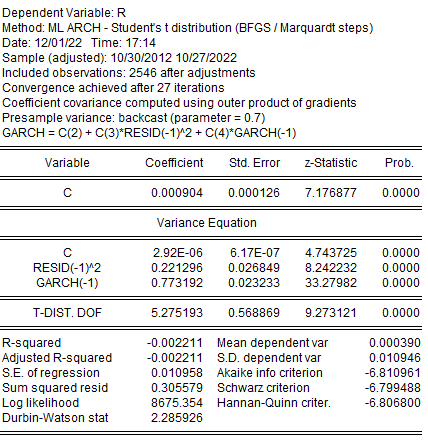
\includegraphics[width=0.6\textwidth]{GARCHt}
\end{center}
The estimated degrees of freedom are 5.28, which corresponds to fairly heavy tails. We then save the GARCH variance series as before, choosing the name \verb.garcht_sig2.. Then we convert the variances into volatilities and compute the VaR, using the commands
\begin{verbatim}
genr garcht_sig = @sqrt(garcht_sig2)
genr var_garch_t = -c(1)-garcht_sig *
                   @sqrt((c(5)-2)/c(5))*@qtdist(0.01, c(5))
\end{verbatim}
Note that the second command should be entered on a single line. Also, \texttt{c(5)} corresponds to the estimated degrees of freedom.
\item The value $\sigma_t=0.014875$ for 10/27/2022 can be obtained from the spreadsheet view of \verb.garcht_sig.. The VaR is then computed as
\begin{align*}
VaR^{0.01}_t&=-\mu-\sigma_t\sqrt{\frac{5.28-2}{5.28}}t^{-1}_{0.01}(5.28)\\
&\approx-0.000904-0.014875\cdot \sqrt{\frac{3.28}{5.28}}\cdot(-3.365)\\
&=0.038547.
\end{align*}
This is an approximation, because $t^{-1}_{0.01}(5.28)$ cannot be obtained from the $t$ distribution table, so we use $t^{-1}_{0.01}(5)=-3.365$. The exact result, 0.037690, can be found in the spreadsheet view for \verb.var_garch_t..

\item The plot below can be generated by opening the four VaR predictions, together with the negative returns, as a group.
\begin{center}
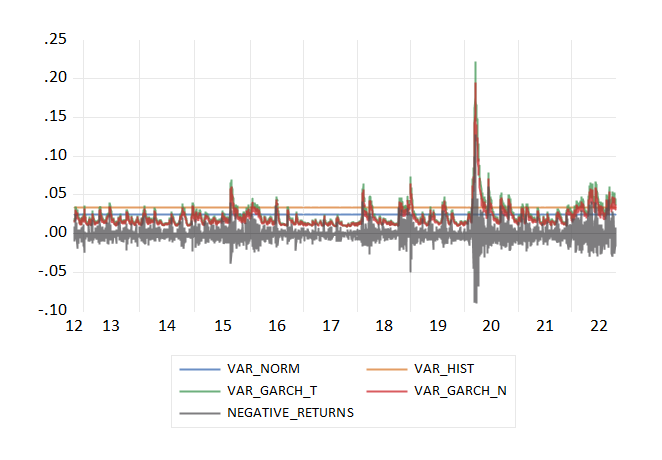
\includegraphics[width=0.8\textwidth]{VaR}
\end{center}
\end{enumerate}
\item The four hit series are generated as follows:
\begin{verbatim}
genr hit_norm = (negative_returns > var_norm)
genr hit_hist = (negative_returns > var_hist)
genr hit_garchn = (negative_returns > var_garch_n)
genr hit_garcht = (negative_returns > var_garch_t)
\end{verbatim}
Each of the hit series will be equal to one at time $t$ if the negative return on that day exceeded the respective VaR estimate. We begin by testing, for each hit series, if the proportion of VaR violations is significantly different from zero. For example, for the historical VaR, this works as follows: compute $\hat{\pi}=T_1/T=\frac{1}{T}\sum_{t=1}^T I_t$ via
\begin{verbatim}
scalar p_hist = @mean(hit_hist)
\end{verbatim}
This yields $\hat{\pi}=0.009819$. From this, we can compute the $t$-statistic
\[
t=\frac{\hat{\pi}-p}{\sqrt{\hat{\pi}(1-\hat{\pi})/T}}=\frac{0.009819-0.01}{\sqrt{0.009819(1-0.009819)/2547}}=-0.09264.
\]
Comparing this with the critical value $\pm 1.96$, we see that $\hat\pi$ is not significantly different from $p$, hence the model has correct unconditional coverage. Note that this is \textbf{by construction}, because we defined the the historical VaR as a sample quantile. So by construction, exactly 1\% of the negative returns should exceed the VaR. Alteratively, we can just regress $I_t-0.01$ onto an intercept by entering the regression specification
\begin{verbatim}
(hit_hist - 0.01) c
\end{verbatim}
and test whether the intercept is significant. The output is
\begin{center}
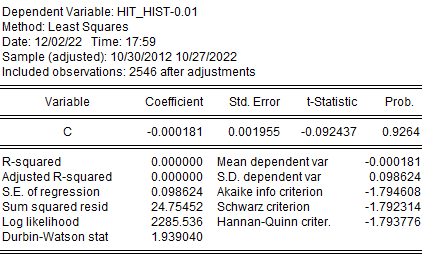
\includegraphics[width=0.6\textwidth]{hit1}
\end{center}
We see that the $t$-statistic obtained this way is almost the same (the two tests are asymptotically equivalent), so we arrive at the same conclusion.

To test for independence, we regress $I_t-0.01$ on an intercept and $I_{t-1}$, by entering the regression specification
\begin{verbatim}
(hit_hist) c hit_hist(-1)
\end{verbatim}
The output is
\begin{center}
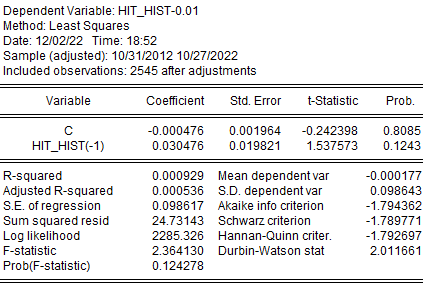
\includegraphics[width=0.6\textwidth]{hit2}
\end{center}
Independence can be tested by checking if $b_1$, the coefficient on the lagged hit, is significant at the 5\% level. Here, surprisingly, it isn't, so we don't reject the null of independence of the VaR violations. Finally, we can use an $F$-test for $H_0:b_0=b_1=0$ to test the correctness of the conditional coverage. Note that we cannot use the $F$-statistic provided in the output above, because that is for a test of the null that all coefficients \emph{except the intercept} are significant. Instead, go to \texttt{View$\rightarrow$Coefficient Diagnostics$\rightarrow$Wald Test}, and enter the restrictions
\begin{verbatim}
c(1)=0, c(2)=0
\end{verbatim}
The result is shown below.
\begin{center}
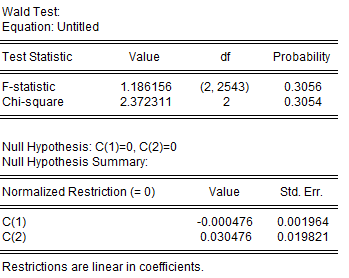
\includegraphics[width=0.6\textwidth]{wald}
\end{center}
The degrees of freedom of the $F$-test are 2 and $T-2$. From the table, we find that the critical value is 3, which is not exceeded by the observed value 1.19. Hence, the null of correct conditional coverage is resoundingly rejected. I should note that this is \textbf{highly unusual}; typically, the historical VaR will fail the independence and conditional coverage tests, because the fact that it doesn't react to changes in volatility means that violations will cluster during crises, making them dependent.

Repeating the analysis for the
other hit series results in the table below.
\begin{center}
\begin{tabular}{l|rrrr}
\toprule
& Hist & Norm &  GARCHn & GARCHt \\ \midrule
$\hat{\pi}\quad (\times 100)$ & $0.98$ & $2.04$ & $2.59$ & $1.65$\\
$t(\pi =0.01)$ & $-0.09$ & $3.72$ & $5.06$ & $2.57$ \\
$\hat{b}_{1}$ & $0.03$ & $0.08$ & $0.00$ & $0.03$\\
$t(b_{1}=0)$ & $1.54$ & $3.91$ & $0.23$ & $1.60$  \\
$F(b_{0}=b_{1}=0)$ & $1.18$ & $14.60$ & $12.80$ & $4.59$\\ \bottomrule
\end{tabular}\\
\end{center}
For the normal VaR, all 3 tests reject. The GARCH models pass the independence test, while the conditional and unconditional coverage tests reject.
\end{enumerate}
\end{document} 